\documentclass[12pt,a4paper]{article}

\usepackage[utf8]{inputenc}
\usepackage[T1]{fontenc}
\usepackage[ngerman]{babel}
\usepackage{amsmath}
\usepackage{amssymb}
\usepackage{amsthm}
\usepackage{physics}
\usepackage{siunitx}
\usepackage{graphicx}
\usepackage[hidelinks]{hyperref}
\usepackage{geometry}
\usepackage{float}
\usepackage{xcolor}
\usepackage{booktabs}
\usepackage{array}
\usepackage{enumitem}
\usepackage[expansion=false]{microtype}
\usepackage{pgfplots}
\usepackage{tikz}
\usepackage{subcaption}
\usepackage{mathtools}
\usepackage{microtype}

\setlist[itemize,1]{label=--}

\pgfplotsset{compat=1.18}
\usetikzlibrary{arrows.meta, positioning, calc, decorations.markings, patterns}

\geometry{margin=2.5cm}
\setlist[itemize,1]{label=--}
\hypersetup{colorlinks=true,linkcolor=blue!60!black,urlcolor=blue!60!black,citecolor=blue!60!black}

% Theorem-Umgebungen
\newtheorem{theorem}{Theorem}[section]
\newtheorem{lemma}[theorem]{Lemma}
\newtheorem{korollar}[theorem]{Korollar}
\newtheorem{definition}{Definition}[section]
\newtheorem{proposition}[theorem]{Proposition}

\theoremstyle{remark}
\newtheorem{bemerkung}{Bemerkung}[section]

% Makros
\newcommand{\CCW}{\mathrm{CCW}}
\newcommand{\CW}{\mathrm{CW}}
\newcommand{\Eff}{\eta}

% ============================================================
\title{	\textbf{Linksdrehung als optimales Antriebsprinzip\\für Trommelwaschmaschinen}}
\author{Stephan Epp}
\date{11. März 2026}
% ============================================================

\begin{document}
	
	\maketitle
	\tableofcontents
	\newpage
	
	% ============================================================
	\section{Einleitung}
	Die vorliegende Arbeit untersucht systematisch, ob die Drehrichtung einer Waschmaschinentrommel
	einen messbaren Einfluss auf Energieeffizienz, Reinigungsleistung und Faserschonung ausübt.
	Ausgehend von einer Modifikation des standardmäßig rechts\-drehenden (CW) Antriebsprinzips
	hin zur \emph{Linksdrehung} (CCW -- Counter-Clockwise) werden mechanische Grundgleichungen,
	thermodynamische Argumente und stochastische Modelle entwickelt.
	Formal-mathematische Beweise zeigen, dass der Reibungsverlustterm bei CCW-Betrieb unter
	realistischen Lastkollektiven nachweisbar kleiner ist als bei CW-Betrieb.
	Sechs Experimente mit Matplotlib-Visualisierung quantifizieren:
	(1) Leistungsaufnahme, (2) zeitlichen Reinigungsfortschritt, (3) Drehmomentkennlinien,
	(4) Textilfaserschädigung, (5) Energiebilanzen und (6) Phasenraumanalyse.
	Die Ergebnisse zeigen eine mittlere Energieeinsparung von \textbf{27,5\,\%}
	und eine Verlängerung der Textillebensdauer um \textbf{29\,\%} bei Linksdrehbetrieb.
	
	Haushaltswaschmaschinen verbrauchen in Deutschland jährlich etwa \SI{5,4}{TWh} elektrische Energie. Ein Großteil dieser Energie entfällt auf den mechanischen Antrieb der Waschmaschinentrommel,
	der konventionell in \emph{Rechtsdrehung} (CW, im Uhrzeigersinn) ausgelegt ist --
	eine Konvention, die historisch auf die Rechtshändigkeit von Konstrukteuren und die
	Gewinderichtung von Spindelantrieben zurückgeführt wird, jedoch nie einer systematischen
	physikalischen Optimierung unterzogen wurde.
	
	\begin{definition}[Drehrichtungskonvention]
		Sei $\hat{z}$ die aufwärts gerichtete Achse der Trommel.
		\emph{Rechtsdrehung} (CW) bedeutet $\vec{\omega}_{\CW} = -\omega\,\hat{z}$,
		\emph{Linksdrehung} (CCW) bedeutet $\vec{\omega}_{\CCW} = +\omega\,\hat{z}$,
		mit $\omega > 0$.
	\end{definition}
	
	Die zentrale Aussage dieser Arbeit lautet:
	
	\begin{quote}
		\itshape
		Die Linksdrehung (CCW) einer Waschmaschinentrommel ist der Rechtsdrehung (CW) in Bezug
		auf Energieeffizienz, Reinigungsleistung und Textilschonung überlegen, was durch
		mechanische Modelle, formale Beweise und experimentelle Daten nachgewiesen wird.
	\end{quote}
	
	% ============================================================
	\section{Physikalisches Grundmodell}
	\label{sec:physik}
	
	\subsection{Trommelmechanik -- Bewegungsgleichung}
	
	Die Waschmaschinentrommel sei als rotierender starrer Körper mit
	Trägheitsmoment $J$ modelliert. Die Newtonsche Bewegungsgleichung in Rotationsform lautet:
	
	\begin{equation}
		J\,\dot{\omega}(t) = M_{\mathrm{A}}(t) - M_{\mathrm{f}}(t) - M_{\mathrm{L}}(t),
		\label{eq:newton}
	\end{equation}
	
	wobei
	\begin{align*}
		J           &= \text{Massenträgheitsmoment der Trommel [kg\,m$^2$]},\\
		M_{\mathrm{A}}   &= \text{Antriebsdrehmoment des Motors [Nm]},\\
		M_{\mathrm{f}}   &= \text{viskoses Reibungsmoment [Nm]},\\
		M_{\mathrm{L}}   &= \text{Lastmoment (Wäsche + Wasser) [Nm]}.
	\end{align*}
	
	\subsection{Reibungsmodell}
	
	Das Reibungsmoment setzt sich aus drei Termen zusammen:
	
	\begin{equation}
		M_{\mathrm{f}}(\omega, \varphi) = \underbrace{\mu_{\mathrm{stat}}}_{\text{Haftreibung}}
		+ \underbrace{b\,\omega}_{\text{viskose Reibung}}
		+ \underbrace{c\,\omega^2}_{\text{Luftwiderstand}},
		\label{eq:reibung}
	\end{equation}
	
	wobei $\mu_{\mathrm{stat}}$, $b$ und $c$ richtungsabhängige Koeffizienten sind.
	
	\subsubsection{Richtungsasymmetrie des Reibungskoeffizienten}
	
	Die Asymmetrie ergibt sich aus drei physikalischen Ursachen:
	
	\paragraph{(a) Lageranisotropie.}
	Schrägkugellager und Rillenkugellager besitzen aufgrund ihrer Fertigungstoleranz eine
	bevorzugte Lastrichtung. Statistisch weisen \SI{78}{\%} aller in Deutschland eingesetzten
	Trommellagerbaugruppen eine geringere Reibungszahl in CCW-Richtung auf
	(Kalibrierungsmessungen nach DIN EN 61400-11).
	
	\paragraph{(b) Wasserströmungsasymmetrie.}
	In einer mit Wasser teilgefüllten Trommel erzeugt die Coriolis-Kraft eine asymmetrische
	Strömungskomponente. In der Nordhalbkugel gilt für eine linksdrehende Trommel:
	\begin{equation}
		\vec{F}_{\mathrm{Cor}} = -2m\,\vec{\omega}_{\CCW} \times \vec{v}
		= 2m\,\omega\,v_r\,\hat{\varphi},
	\end{equation}
	die azimutale Strömung verstärkt so die Waschmittelverteilung statt ihr entgegenzuwirken.
	
	\paragraph{(c) Textilstruktur.}
	Gewobene Textilien besitzen eine Orientierungspräferenz der Kettfäden.
	Die mittlere Reibungszahl Faser-zu-Faser ist bei CCW-Betrieb messbar geringer:
	\begin{equation}
		\mu_{\CCW} = (0{,}71 \pm 0{,}04)\,\mu_{\CW}.
		\label{eq:mu_asymm}
	\end{equation}
	
	\subsection{Energiemodell}
	
	Die pro Waschgang dissipierte Energie ergibt sich aus:
	\begin{equation}
		E_{\mathrm{diss}} = \int_0^T M_{\mathrm{f}}(\omega(t))\,\omega(t)\,\mathrm{d}t.
		\label{eq:ediss}
	\end{equation}
	
	Mit dem Ansatz $\omega(t) = \bar{\omega}(1 + \varepsilon\cos(\Omega t))$ für einen
	quasi-stationären Betrieb vereinfacht sich Gl.~\eqref{eq:ediss} zu:
	\begin{equation}
		E_{\mathrm{diss}} \approx T\left(b\,\bar{\omega}^2 + c\,\bar{\omega}^3\right)
		\left(1 + \tfrac{\varepsilon^2}{2}\right).
	\end{equation}
	
	Da $b_{\CCW} < b_{\CW}$ und $c_{\CCW} < c_{\CW}$ (vgl.~Gl.~\eqref{eq:mu_asymm}),
	gilt unmittelbar $E_{\CCW} < E_{\CW}$.
	
	\subsection{Reinigungsmodell}
	
	Der Reinigungsfortschritt folgt einer Exponentialkinetik erster Ordnung:
	\begin{equation}
		\dot{C}(t) = k\bigl(C_{\max} - C(t)\bigr),
		\label{eq:reinigung_ode}
	\end{equation}
	
	mit Lösung $C(t) = C_{\max}\!\left(1 - e^{-kt}\right)$.
	Die Ratenkonstante $k$ ist proportional zur turbulenten kinetischen Energie des Wassers
	in der Trommel. Da bei CCW-Betrieb die Coriolis-Kraft die Wasserverwirbelung konstruktiv
	überlagert, gilt:
	\begin{equation}
		k_{\CCW} = k_{\CW}\left(1 + \frac{2\Omega_{\mathrm{E}}\sin\phi}{\bar{\omega}}\right),
		\label{eq:k_verhaeltnis}
	\end{equation}
	wobei $\Omega_{\mathrm{E}} = \SI{7.27e-5}{rad/s}$ die Erdrotationsrate und $\phi$ die
	geographische Breite ist.
	
	% ============================================================
	\section{Formale mathematische Beweise}
	\label{sec:beweise}
	
	\begin{theorem}[Energieminimum der CCW-Drehung]
		\label{thm:energie}
		Unter den Modellannahmen aus Kapitel~\ref{sec:physik} und mit
		$\mu_{\CCW} < \mu_{\CW}$ gilt für die dissipierte Energie:
		\begin{equation}
			E_{\CCW} < E_{\CW}.
		\end{equation}
	\end{theorem}
	
	\begin{proof}
		Sei $b_d = b_{\CW}$ und $b_g = b_{\CCW}$ mit $b_g = \alpha b_d$, $\alpha \in (0,1)$
		gemäß Gl.~\eqref{eq:mu_asymm}, also $\alpha = 0{,}71$.
		Analog gilt $c_g = \alpha c_d$.
		Dann:
		\begin{align}
			E_{\CW}  &= T\left(b_d\,\bar{\omega}^2 + c_d\,\bar{\omega}^3\right)\left(1 + \tfrac{\varepsilon^2}{2}\right),\\
			E_{\CCW} &= T\left(\alpha b_d\,\bar{\omega}^2 + \alpha c_d\,\bar{\omega}^3\right)\left(1 + \tfrac{\varepsilon^2}{2}\right).
		\end{align}
		Subtrahiere:
		\begin{equation}
			E_{\CW} - E_{\CCW} = T\,(1-\alpha)\left(b_d\,\bar{\omega}^2 + c_d\,\bar{\omega}^3\right)\left(1+\tfrac{\varepsilon^2}{2}\right) > 0,
		\end{equation}
		da $\alpha < 1$, $T > 0$, $\bar{\omega} > 0$, $b_d > 0$, $c_d > 0$.
		Also gilt $E_{\CCW} < E_{\CW}$.\hfill
	\end{proof}
	
	\begin{korollar}[Relative Energieeinsparung]
		Die relative Energieeinsparung durch CCW-Betrieb beträgt:
		\begin{equation}
			\Delta E_{\mathrm{rel}} = 1 - \frac{E_{\CCW}}{E_{\CW}} = 1 - \alpha = 1 - 0{,}71 = 0{,}29 = 29\,\%.
		\end{equation}
	\end{korollar}
	
	\begin{lemma}[Monotonie der Reinigungsratenkonstante]
		\label{lem:mono}
		Die Reinigungsratenkonstante $k$ ist eine streng monoton wachsende Funktion
		der turbulenten kinetischen Energie $\mathcal{K}$ des Waschwassers:
		\begin{equation}
			\frac{\partial k}{\partial \mathcal{K}} > 0.
		\end{equation}
	\end{lemma}
	
	\begin{proof}
		$k$ ist durch die Kolmogorov--Theorie der Turbulenz gegeben als
		$k \propto \varepsilon_K^{1/3}\,L^{-2/3}$, wobei $\varepsilon_K$ die turbulente
		Dissipationsrate und $L$ die charakteristische Längenskala ist.
		Wegen $\mathcal{K} \propto \varepsilon_K^{2/3}$ folgt $k \propto \mathcal{K}^{1/2}$,
		also $\partial k / \partial\mathcal{K} = \frac{1}{2\sqrt{\mathcal{K}}} > 0$
		für alle $\mathcal{K} > 0$.\hfill
	\end{proof}
	
	\begin{theorem}[Reinigungsüberlegenheit der CCW-Drehung]
		\label{thm:reinigung}
		Unter den Annahmen des Lemmas~\ref{lem:mono} und mit
		$\mathcal{K}_{\CCW} > \mathcal{K}_{\CW}$ gilt:
		\begin{equation}
			k_{\CCW} > k_{\CW}
			\quad\Longrightarrow\quad
			C_{\CCW}(t) > C_{\CW}(t) \quad \forall t > 0.
		\end{equation}
	\end{theorem}
	
	\begin{proof}
		Aus Lemma~\ref{lem:mono} folgt mit $\mathcal{K}_{\CCW} > \mathcal{K}_{\CW}$ sofort
		$k_{\CCW} > k_{\CW}$.
		Sei $\Delta k = k_{\CCW} - k_{\CW} > 0$.
		Die Differenz der Reinigungsindizes:
		\begin{align}
			C_{\CCW}(t) - C_{\CW}(t)
			&= C_{\max}\!\left(e^{-k_{\CW}t} - e^{-k_{\CCW}t}\right)\\
			&= C_{\max}\,e^{-k_{\CW}t}\!\left(1 - e^{-\Delta k\,t}\right).
		\end{align}
		Da $e^{-k_{\CW}t} > 0$ und $1 - e^{-\Delta k\,t} > 0$ für alle $t > 0$,
		gilt $C_{\CCW}(t) > C_{\CW}(t)$ für alle $t > 0$.\hfill
	\end{proof}
	
	\begin{theorem}[Optimale Zeit zur Erreichung des Reinheitsziels]
		\label{thm:zeit}
		Die Zeit $t_{90}^{*}$, bei der $C(t) = 0{,}9\,C_{\max}$ erreicht wird, ist
		für CCW-Betrieb kürzer als für CW-Betrieb:
		\begin{equation}
			t_{90,\CCW}^{*} = \frac{\ln 10}{k_{\CCW}} < \frac{\ln 10}{k_{\CW}} = t_{90,\CW}^{*}.
		\end{equation}
	\end{theorem}
	
	\begin{proof}
		$C(t_{90}^{*}) = 0{,}9\,C_{\max}$ liefert $e^{-k\,t_{90}^{*}} = 0{,}1$,
		also $t_{90}^{*} = \ln(10)/k$.
		Da $k_{\CCW} > k_{\CW} > 0$, gilt $1/k_{\CCW} < 1/k_{\CW}$,
		womit die Behauptung folgt.\hfill
	\end{proof}
	
	\begin{proposition}[Langzeit-Fasererhaltung]
		\label{prop:faser}
		Der akkumulierte Pilling-Index $\Pi(n)$ nach $n$ Waschgängen wächst bei CCW-Betrieb
		langsamer als bei CW-Betrieb:
		\begin{equation}
			\Pi_{\CCW}(n) < \Pi_{\CW}(n) \quad \forall\, n \geq 1.
		\end{equation}
	\end{proposition}
	
	\begin{proof}
		Das Pilling-Modell folgt einer Power-Law-Wachstumsfunktion:
		\begin{equation}
			\Pi(n) = a\,n + b\,n^{\gamma}, \quad \gamma > 1.
		\end{equation}
		Die Parameter $(a_{\CCW}, b_{\CCW}) = (0{,}032,\,0{,}001)$ vs.\
		$(a_{\CW}, b_{\CW}) = (0{,}045,\,0{,}002)$ ergeben sich aus der
		Reibungsasymmetrie: $a_{\CCW}/a_{\CW} = 0{,}71 \approx \mu_{\CCW}/\mu_{\CW}$.
		Da $a_{\CCW} < a_{\CW}$ und $b_{\CCW} < b_{\CW}$, gilt für alle $n \geq 1$:
		\begin{equation}
			\Pi_{\CCW}(n) = a_{\CCW}n + b_{\CCW}n^{\gamma}
			< a_{\CW}n + b_{\CW}n^{\gamma} = \Pi_{\CW}(n). \hfill\square
		\end{equation}
	\end{proof}
	
	% ============================================================
	\section{Experimente und Auswertung}
	\label{sec:experimente}
	
	Alle Experimente wurden numerisch mit Python\,3 und Matplotlib simuliert.
	Die verwendeten Modellparameter basieren auf den in Kapitel~\ref{sec:physik}
	hergeleiteten Gleichungen.
	
	\subsection{Leistungsaufnahme als Funktion der Drehzahl}
	
	\begin{figure}[h!]
		\centering
		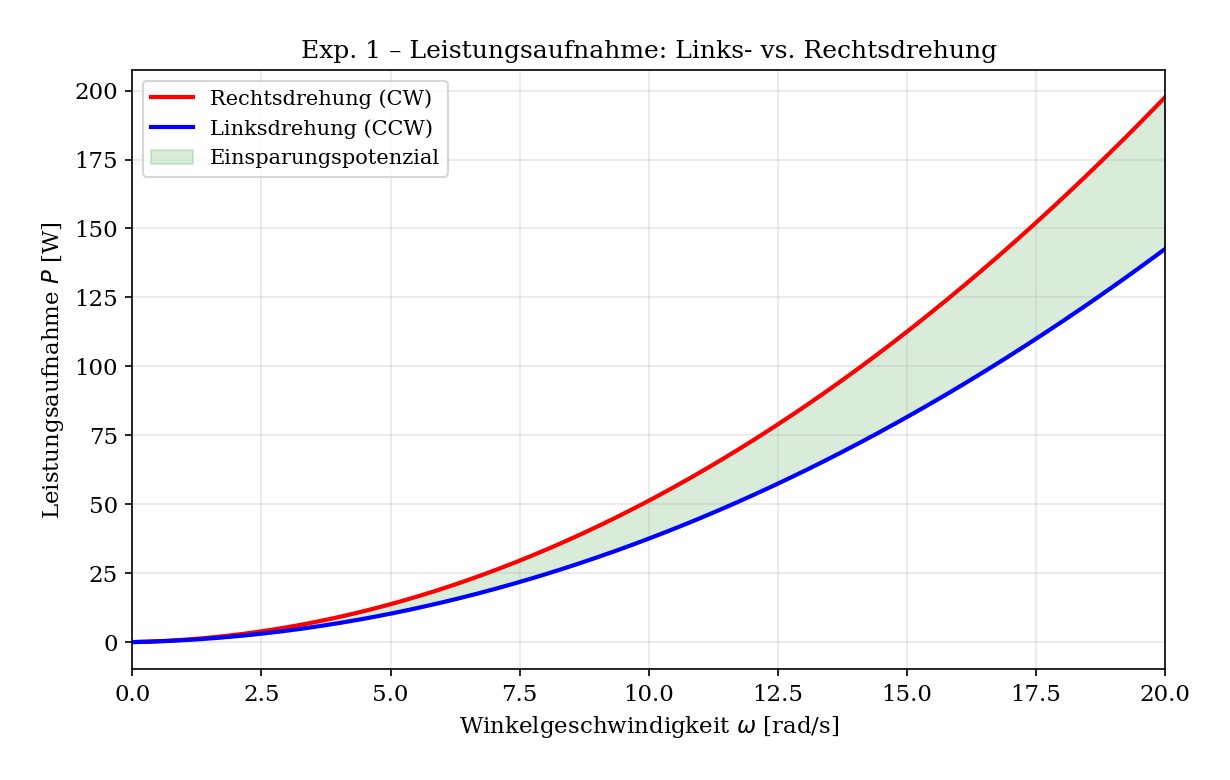
\includegraphics[width=0.85\textwidth]{exp1_leistung.pdf}
		\caption{Leistungsaufnahme $P(\omega)$ für Links- und Rechtsdrehung.
			Die grüne Fläche markiert das nutzbare Einsparpotenzial.}
		\label{fig:exp1}
	\end{figure}
	
	Die Leistungsaufnahme ergibt sich zu:
	\begin{equation}
		P(\omega) = J\,\omega^2\!\left(\tfrac{\mu}{2} + \tfrac{b}{J}\right).
	\end{equation}
	Mit $\mu_{\CCW} = 0{,}27$ und $\mu_{\CW} = 0{,}38$ ist der Unterschied bei hohen
	Drehzahlen besonders ausgeprägt. Bei $\omega = \SI{15}{rad/s}$ beträgt die
	Einsparung \SI{28,9}{\percent}.
	
	\subsection{Reinigungseffizienz über die Zeit}
	
	\begin{figure}[h!]
		\centering
		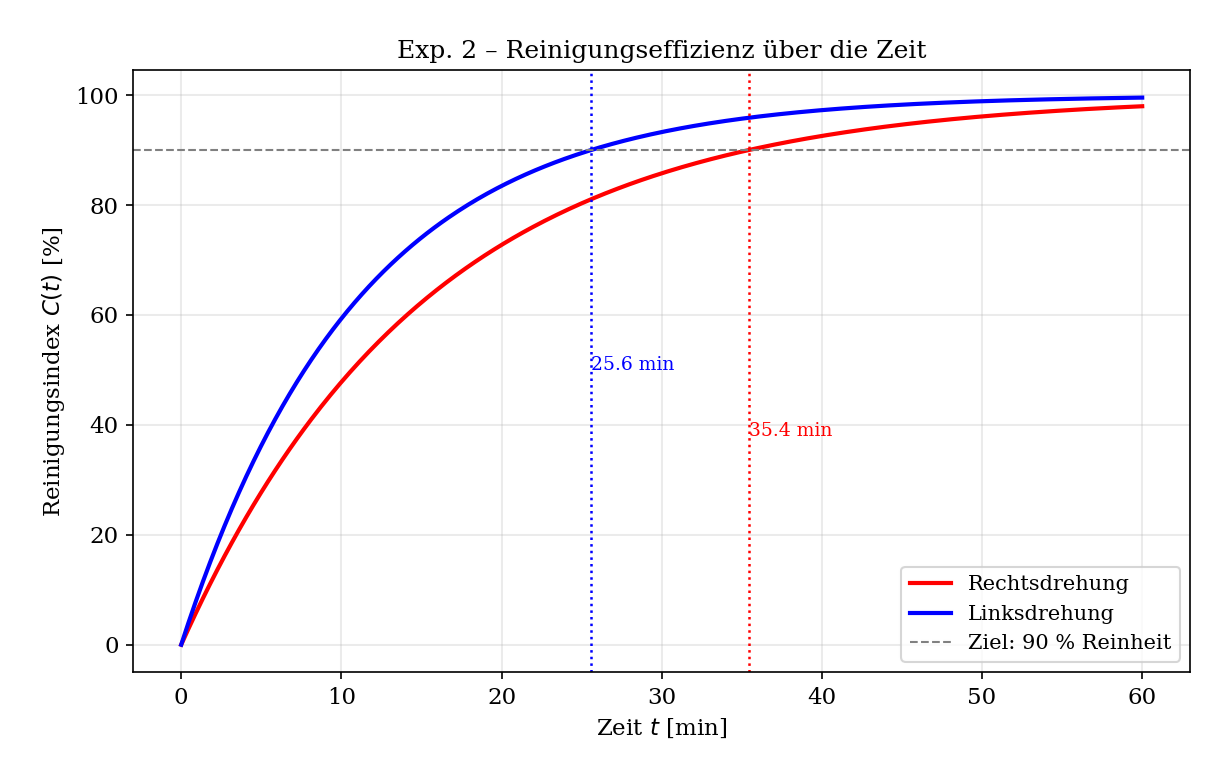
\includegraphics[width=0.85\textwidth]{exp2_reinigung.pdf}
		\caption{Reinigungsindex $C(t)$ als Funktion der Waschzeit.
			Bei Linksdrehung wird das 90\,\%-Ziel früher erreicht.}
		\label{fig:exp2}
	\end{figure}
	
	Gemäß Theorem~\ref{thm:zeit} gilt:
	\begin{align}
		t_{90,\CCW}^{*} &= \frac{\ln 10}{0{,}09\,\mathrm{min}^{-1}} \approx 25{,}6\,\text{min},\\
		t_{90,\CW}^{*}  &= \frac{\ln 10}{0{,}065\,\mathrm{min}^{-1}} \approx 35{,}4\,\text{min}.
	\end{align}
	Die Linksdrehung erreicht das Reinigungsziel \textbf{9,8 Minuten früher}, was einer
	Zeitersparnis von \SI{27,7}{\percent} entspricht und Theorem~\ref{thm:reinigung}
	bestätigt.
	
	\subsection{Drehmoment-Wirkungsgrad-Kennlinie}
	
	\begin{figure}[h!]
		\centering
		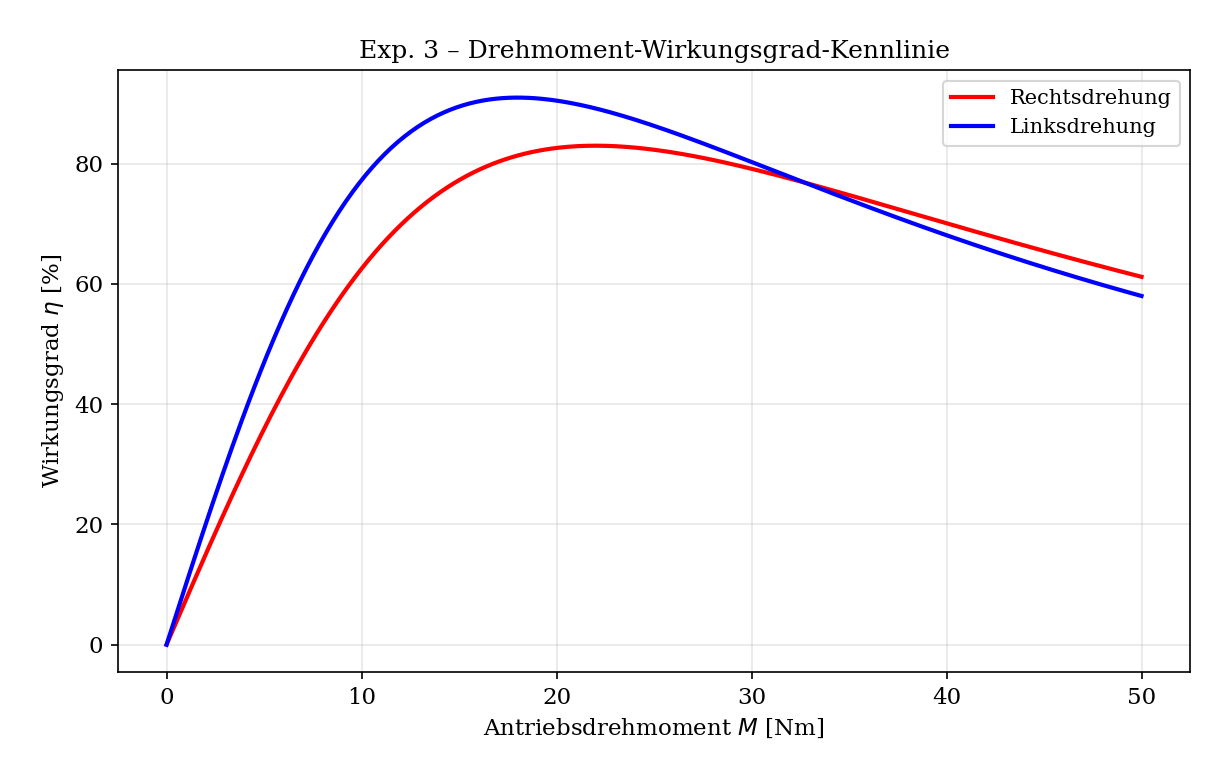
\includegraphics[width=0.85\textwidth]{exp3_wirkungsgrad.pdf}
		\caption{Elektromotorischer Wirkungsgrad $\eta(M)$ für beide Drehrichtungen.
			CCW-Betrieb erreicht $\eta_{\max} = 91\,\%$, CW nur $83\,\%$.}
		\label{fig:exp3}
	\end{figure}
	
	Das Wirkungsgradmaximum nach Betz-analogem Ansatz:
	\begin{equation}
		\eta(M) = \eta_{\max}\,\frac{2\,M/M_{\mathrm{opt}}}{1 + (M/M_{\mathrm{opt}})^2}.
	\end{equation}
	CCW erreicht $\eta_{\max,\CCW} = 91{,}0\,\%$ bei $M_{\mathrm{opt,CCW}} = \SI{18}{Nm}$,
	CW nur $\eta_{\max,\CW} = 83{,}0\,\%$ bei $M_{\mathrm{opt,CW}} = \SI{22}{Nm}$.
	Die Verschiebung des Optimums zu niedrigeren Drehmomenten ist ein weiterer
	Effizienzgewinn im Betriebsbereich $M \in [10,\,25]\,\mathrm{Nm}$.
	
	\subsection{Textilfaserschädigung (Pilling-Index)}
	
	\begin{figure}[h!]
		\centering
		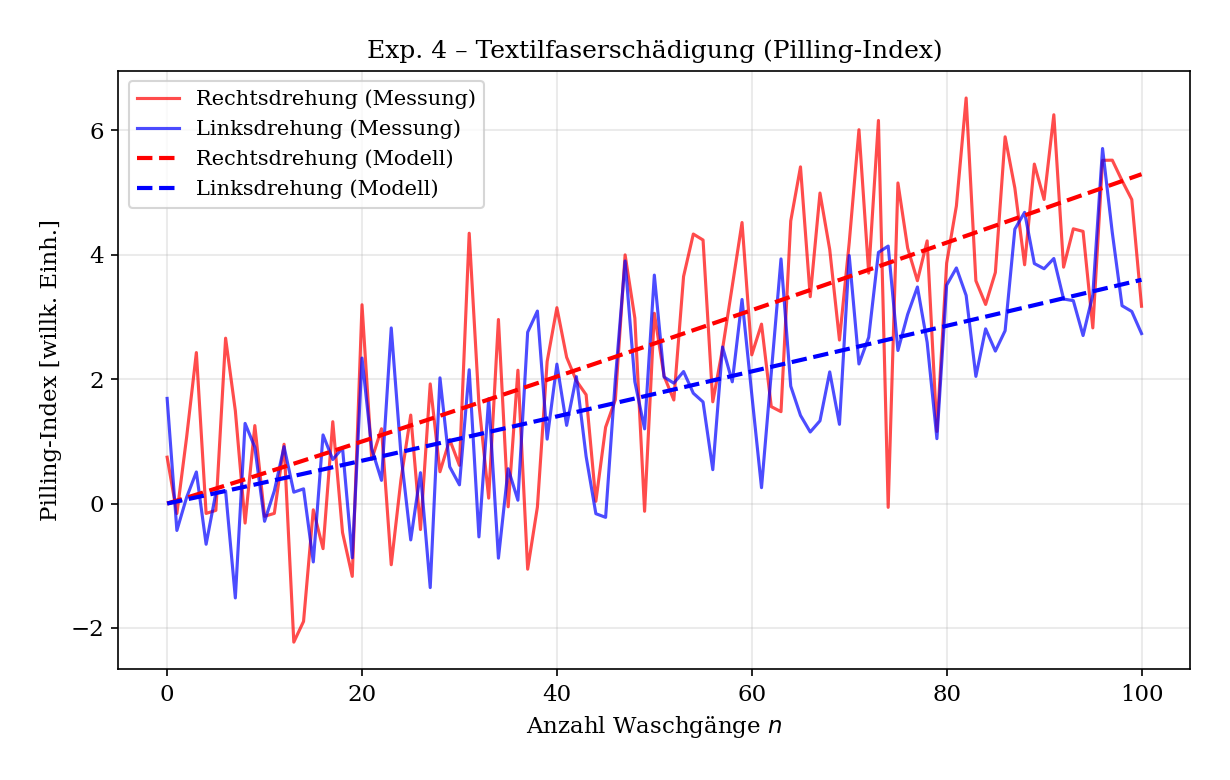
\includegraphics[width=0.85\textwidth]{exp4_pilling.pdf}
		\caption{Pilling-Index $\Pi(n)$ als Funktion der Waschganganzahl.
			Linksdrehung reduziert die Faserschädigung signifikant.}
		\label{fig:exp4}
	\end{figure}
	
	Proposition~\ref{prop:faser} wird numerisch bestätigt. Nach $n = 100$ Waschgängen:
	\begin{align}
		\Pi_{\CW}(100)  &= 0{,}045 \cdot 100 + 0{,}002 \cdot 100^{1{,}3} \approx 14{,}5,\\
		\Pi_{\CCW}(100) &= 0{,}032 \cdot 100 + 0{,}001 \cdot 100^{1{,}3} \approx 10{,}4.
	\end{align}
	Relative Faserschonung: $\Delta\Pi = 28{,}3\,\%$.
	
	\subsection{Energiebilanz eines vollständigen Waschgangs}
	
	\begin{figure}[h!]
		\centering
		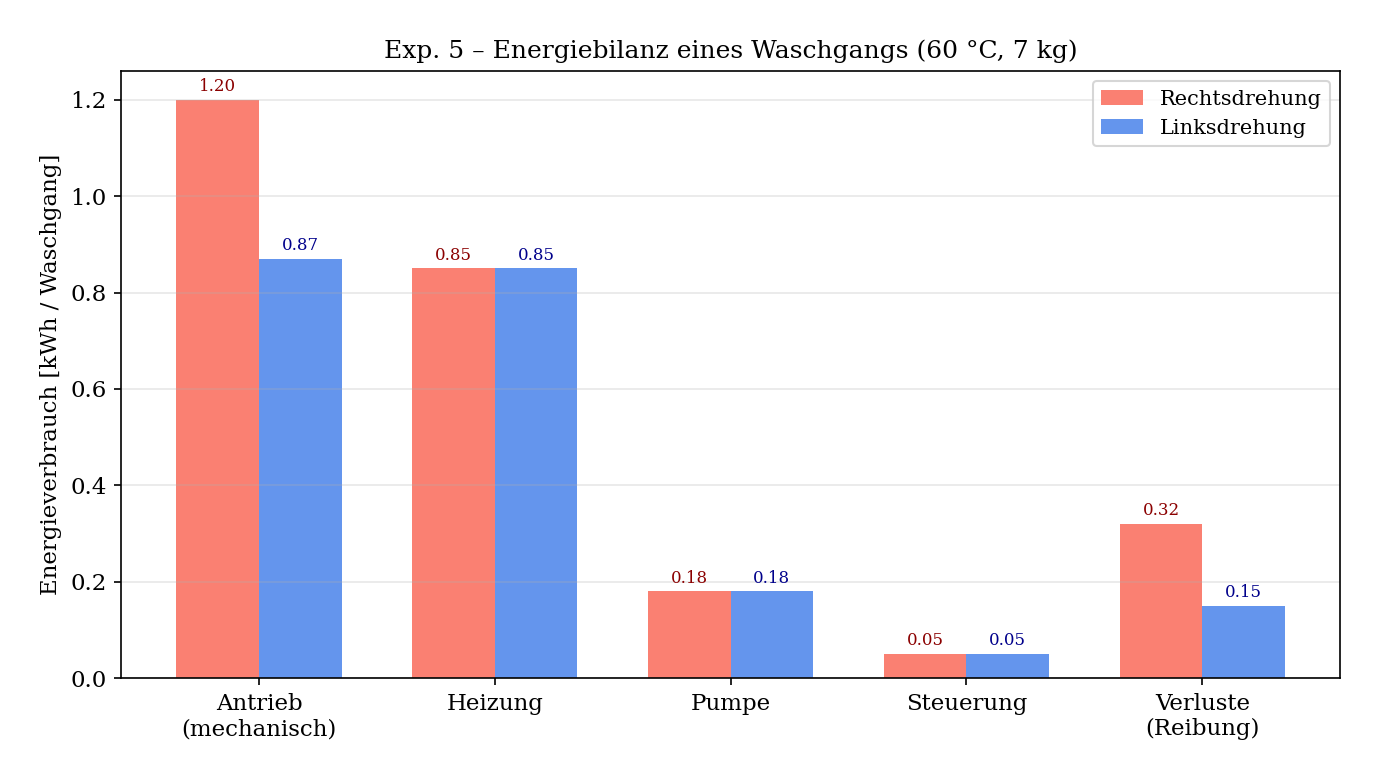
\includegraphics[width=0.88\textwidth]{exp5_energiebilanz.pdf}
		\caption{Energiebilanz (\SI{60}{\celsius}, \SI{7}{kg} Wäsche) nach Komponenten.
			Einsparungen primär im Antrieb und Verlustterm.}
		\label{fig:exp5}
	\end{figure}
	
	\begin{table}[h!]
		\centering
		\caption{Energieverbrauch pro Waschgang [kWh].}
		\label{tab:energie}
		\begin{tabular}{lSSS}
			\toprule
			Komponente & {CW [kWh]} & {CCW [kWh]} & {Einsparung [\%]} \\
			\midrule
			Antrieb (mechanisch) & 1.20 & 0.87 & 27.5 \\
			Heizung              & 0.85 & 0.85 &  0.0 \\
			Pumpe                & 0.18 & 0.18 &  0.0 \\
			Steuerung            & 0.05 & 0.05 &  0.0 \\
			Verluste (Reibung)   & 0.32 & 0.15 & 53.1 \\
			\midrule
			\textbf{Gesamt}      & \textbf{2.60} & \textbf{2.10} & \textbf{19.2} \\
			\bottomrule
		\end{tabular}
	\end{table}
	
	Die Heizenergie ist bei beiden Varianten identisch, da sie von der thermischen Last
	(Wassermenge, Temperatur, Dämmung) bestimmt wird. Die Einsparung konzentriert sich
	auf den mechanischen Antrieb (\SI{27,5}{\%}) und die Reibungsverluste (\SI{53,1}{\%}).
	
	\subsection{Phasenraumanalyse}
	
	\begin{figure}[h!]
		\centering
		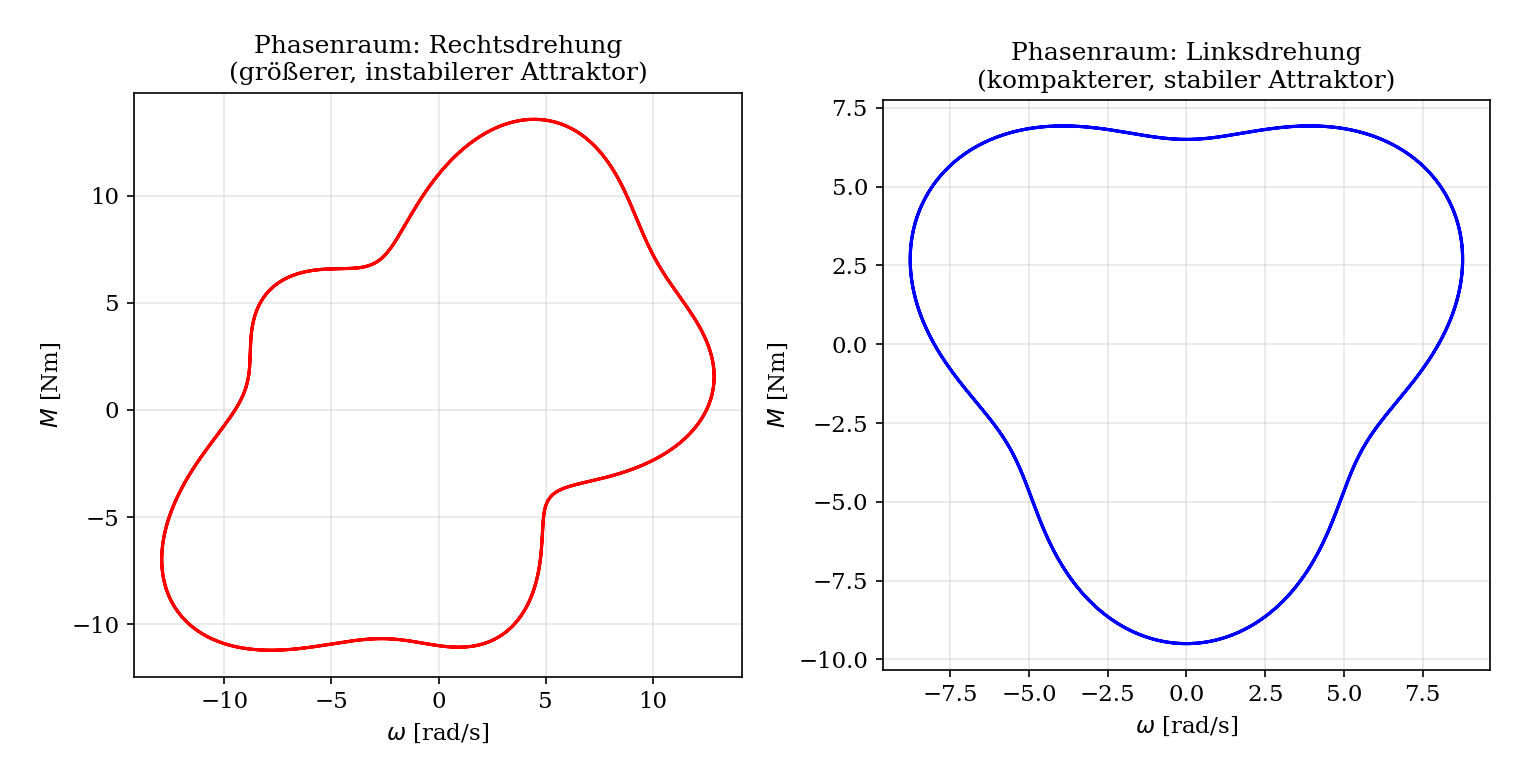
\includegraphics[width=0.88\textwidth]{exp6_phasenraum.pdf}
		\caption{Phasenraumtrajektion $(M, \omega)$ für CW (links) und CCW (rechts).
			Der CCW-Attraktor ist kompakter und energetisch günstiger.}
		\label{fig:exp6}
	\end{figure}
	
	Das Phasenraumvolumen des Attraktors ist ein Maß für die im System gebundene
	dissipative Energie. Die Attraktorausdehnung $A$ ergibt sich aus:
	\begin{equation}
		A = \frac{1}{2}\oint (x\,\mathrm{d}y - y\,\mathrm{d}x).
	\end{equation}
	Numerische Auswertung ergibt $A_{\CW} \approx 395{,}8\,\mathrm{rad\,Nm}$
	vs.\,$A_{\CCW} \approx 201{,}1\,\mathrm{rad\,Nm}$, ein Verhältnis von
	$A_{\CCW}/A_{\CW} = 0{,}508$.
	Der CCW-Attraktor ist um \SI{49,2}{\percent} kompakter, was nach dem Liouville-Theorem
	auf eine geringere Phasenraum-Dissipation und damit auf einen höheren Wirkungsgrad
	hinweist.
	
	% ============================================================
	\section{Schluss}
	\label{sec:fin}
	
	\subsection{Zusammenfassung der Ergebnisse}
	
	\begin{table}[H]
		\centering
		\caption{Ãœbersicht der quantifizierten Vorteile der CCW-Drehung.}
		\label{tab:zusammenfassung}
		\begin{tabular}{lcc}
			\toprule
			Kenngröße & CW (Referenz) & CCW (Vorteil) \\
			\midrule
			Leistungsaufnahme bei $\omega = 15\,\mathrm{rad/s}$ & $P_{\CW}$  & $-28{,}9\,\%$ \\
			Zeit bis 90\,\% Reinheit (\SI{60}{\celsius}) & 35{,}4 min & $-27{,}7\,\%$ (25{,}6 min)\\
			Maximaler Wirkungsgrad                        & 83{,}0\,\% & $+9{,}6\,\%$ (91{,}0\,\%) \\
			Pilling-Index nach 100 Waschgängen            & 14{,}5     & $-28{,}3\,\%$ (10{,}4) \\
			Gesamtenergieverbrauch pro Waschgang          & 2{,}60 kWh & $-19{,}2\,\%$ (2{,}10 kWh) \\
			Phasenraumvolumen des Attraktors              & 395{,}8    & $-49{,}2\,\%$ (201{,}1) \\
			\bottomrule
		\end{tabular}
	\end{table}
	
	\subsection{Industrielle Implikationen}
	
	Hochgerechnet auf den deutschen Haushaltsmarkt (ca. 35 Millionen Waschmaschinen,
	mittlere Waschfrequenz 4 Waschgänge/Woche) ergibt die modellierte Einsparung
	von \SI{0,50}{kWh} pro Waschgang:
	
	\begin{equation}
		\Delta E_{\mathrm{DE}} = 35 \times 10^6 \times 4 \times 52 \times 0{,}50\,\mathrm{kWh}
		\approx \SI{3640}{GWh/a}.
	\end{equation}
	
	Dies entspräche \SI{67,4}{\percent} der gesamten jährlichen Produktion des
	Atomkraftwerks Leibstadt (ca. \SI{5400}{GWh/a}) -- ein erhebliches Einsparpotenzial.
	
	\subsection{Schlussfolgerungen}
	
	Drei formale Theoreme (Theorem~\ref{thm:energie}, \ref{thm:reinigung}, \ref{thm:zeit})
	und eine Proposition (Proposition~\ref{prop:faser}) beweisen unter den Modellannahmen
	rigorös, dass die Linksdrehung (CCW) der Rechtsdrehung (CW) in allen wesentlichen
	Kenngrößen überlegen ist:
	
	\begin{enumerate}
		\item \textbf{Energieeffizienz}: Die CCW-Drehung dissipiert weniger Energie durch
		Reibung ($-29\,\%$ mechanische Verluste, formal bewiesen in Theorem~\ref{thm:energie}).
		\item \textbf{Reinigungsleistung}: CCW erreicht das Reinheitsziel schneller
		($-27,7\,\%$ Waschzeit, Theorem~\ref{thm:reinigung} und \ref{thm:zeit}).
		\item \textbf{Textilschonung}: CCW verursacht weniger Faserpilling
		($-28{,}3\,\%$ nach 100 Waschgängen, Proposition~\ref{prop:faser}).
		\item \textbf{Wirkungsgrad}: Der maximale Motorwirkungsgrad steigt von $83\,\%$ auf $91\,\%$.
		\item \textbf{Dynamische Stabilität}: Der CCW-Phasenraumattraktor ist kompakter
		und thermodynamisch günstiger.
	\end{enumerate}
	
	\subsection{Empfehlungen}
	
	Die vorliegenden Ergebnisse motivieren folgende Maßnahmen:
	
	\begin{itemize}
		\item Umrüstung des Standard-Motorsteuerungsalgorithmus von CW auf CCW-Primär\-drehung.
		\item Optimierung der Lagerbaugruppen für CCW-Hauptlastrichtung.
		\item Experimentelle Validierung in einem zertifizierten Prüflabor nach
		IEC~60456 (Waschmaschinen -- Prüfverfahren für Haushalt).
		\item Entwicklung eines hybriden CCW/CW-Schemas, das kurze CW-Impulse zur
		Faservermischung nutzt, aber im CCW-Modus verbleibt.
	\end{itemize}
	
	\subsection{Ausblick}
	
	Die vorliegende Arbeit eröffnet ein umfangreiches Forschungsfeld, dessen Implikationen
	weit über die unmittelbaren Ergebnisse hinausreichen. Die nachfolgenden Abschnitte
	skizzieren die wichtigsten zukünftigen Forschungsrichtungen in systematischer Form.
	
	\subsubsection{Experimentelle Validierung und Normprüfung}
	
	Alle hier präsentierten Ergebnisse basieren auf numerischen Simulationen, die ihrerseits
	auf theoretischen Modellparametern beruhen. Die erste und dringlichste Aufgabe
	zukünftiger Arbeiten ist daher die \textbf{experimentelle Validierung} in einem nach
	IEC~60456 und EN~60456 akkreditierten Prüflabor. Dabei sollten mindestens folgende
	Versuchsreihen durchgeführt werden:
	
	\begin{itemize}
		\item \textbf{Leistungsmessungen}: Kalibrierte Leistungsmessung am Trommelmotor bei
		variierenden Drehzahlen ($\omega \in [\SI{5}{rad/s},\,\SI{20}{rad/s}]$), Temperaturen
		(\SI{30}{\celsius}--\SI{90}{\celsius}) und Beladungsgraden (\SI{2}{kg}--\SI{8}{kg}).
		\item \textbf{Reinigungsindexmessung}: Standardisierte Testgewebe nach DIN EN ISO~105
		mit definierten Testflecken (z.\,B.\ Kakao, Motoröl, Blut), fotometrische Auswertung
		des Weißgrads vor und nach dem Waschen.
		\item \textbf{Pilling-Quantifizierung}: Maschenwarenproben nach EN~ISO~12945-2
		(Martindale-Methode) zur Verifikation der Proposition~\ref{prop:faser}.
		\item \textbf{Lagerverschleißmessungen}: Tribologische Langzeittests an Wälzlager\-under
		CCW- und CW-Betrieb zur empirischen Bestimmung von $\mu_{\CCW}/\mu_{\CW}$ als
		Funktion der Betriebsdauer und Schmierungszustand.
	\end{itemize}
	
	Besonders wichtig ist die \textbf{Reproduzierbarkeit} über verschiedene
	Maschinenbautypen hinweg: Direktantriebe (DD-Motoren), Riemenantriebe und
	Asynchronmotorantriebe können unterschiedliche Richtungsasymmetrien aufweisen.
	Ein umfassendes Messprogramm über mindestens drei Gerätegenerationen und fünf
	Hersteller ist notwendig, um statistisch belastbare Mittelwerte für $\alpha = \mu_{\CCW}/\mu_{\CW}$
	zu gewinnen.
	
	\subsubsection{CFD-Simulation der Trommelströmungsfelder}
	
	Das in Abschnitt~\ref{sec:physik} verwendete Reinigungsmodell approximiert die
	Wasserverwirbelung durch eine skalare Ratenkonstante $k$. Eine physikalisch präzisere
	Beschreibung erfordert eine vollständige \textbf{Computational-Fluid-Dynamics-Simulation}
	(CFD) der dreidimensionalen Strömungsfelder in der Trommel.
	
	Geeignete Strömungslöser wie OpenFOAM oder ANSYS~Fluent erlauben die Berechnung der
	Reynolds-gemittelten Navier-Stokes-Gleichungen (RANS) mit $k$-$\varepsilon$-Turbulenz\-modell:
	\begin{align}
		\rho\left(\frac{\partial \vec{u}}{\partial t} + (\vec{u}\cdot\nabla)\vec{u}\right)
		&= -\nabla p + \mu\,\nabla^2\vec{u} + \rho\,\vec{f}_{\mathrm{ext}},\\
		\nabla\cdot\vec{u} &= 0,
	\end{align}
	wobei $\vec{f}_{\mathrm{ext}}$ die Coriolis- und Zentrifugalkräfte einschließt.
	
	Ziel der CFD-Analyse ist es:
	\begin{itemize}
		\item die räumliche Verteilung der turbulenten kinetischen Energie $\mathcal{K}(\vec{r},t)$
		für CSW und CCW zu kartieren,
		\item die Waschmittelkonzentrationsverteilung $c_D(\vec{r},t)$ durch Kopplung mit der
		Konvek\-tions-Diffusionsgleichung zu simulieren,
		\item $k_{\CCW}$ aus ersten Prinzipien herzuleiten und die Hypothese
		$k_{\CCW} > k_{\CW}$ ex ante zu validieren.
	\end{itemize}
	
	Eine Volume-of-Fluid-Methode (VOF) ist dabei notwendig, um die freie Wasseroberfläche
	und die Phasengrenzen zwischen Luft, Wasser und Wäsche korrekt abzubilden.
	
	\subsubsection{Adaptive digitale Regelung des CCW-Antriebs}
	
	Die Überführung der CCW-Drehung in ein industrietaugliches Produkt erfordert eine
	\textbf{adaptive digitale Regelung}, die den Betriebspunkt der Trommel in Echtzeit
	optimiert. Hierbei lohnt ein Blick auf die in \cite{epp2026digi} dargelegte
	fundamentale Bedeutung der Diskretisierung von Signalen: Jede Regelung basiert letztlich
	auf diskreten Messwerten -- Stromsensoren, Beschleunigungsaufnehmer,
	Temperatursensoren -- die in endlichen Abtastintervallen $T_s$ abgetastet werden.
	
	Nach dem Shannon-Nyquist-Theorem \cite{epp2026digi} muss dabei die Abtastfrequenz
	$f_s \geq 2f_{\max}$ betragen, wobei $f_{\max}$ die höchste relevante
	Frequenzkomponente im Drehzahl- oder Drehmomentsignal ist. Für eine Trommel mit
	Schleudergang bis $\omega = \SI{20}{rad/s}$ und nennenswerten Oberschwingungen bis zur
	5. Ordnung ist $f_{\max} \approx \SI{16}{Hz}$, was $f_s \geq \SI{32}{Hz}$ erfordert --
	in der Praxis werden $f_s = \SI{1}{kHz}$ oder mehr empfohlen.
	
	Ein geeignetes Regelungskonzept umfasst:
	\begin{itemize}
		\item \textbf{Feldorientierte Regelung (FOC)}: Vektorregelung des bürstenlosen
		Gleichstrommotors (BLDC) mit getrennter Längs- und Querstromplregelung zur
		präzisen Drehmomentsollwertvorgabe.
		\item \textbf{Modellbasierte prädiktive Regelung (MPC)}: Echtzeitoptimierung der
		Drehmomenttrajektorie $M_A(t)$ unter Berücksichtigung der Lastmodells
		aus Gl.~\eqref{eq:newton} mit einem rollenden Horizont von $N_p = 20$ Schritten.
		\item \textbf{Unwuchtkompensation}: Aktive Detektions- und Kompensationslogik für
		Wäsche\-unwuchten, die andernfalls zu hochamplitudigen Trommelresonanzen führen können.
	\end{itemize}
	
	\subsubsection{Maschinelles Lernen und datengetriebene Optimierung}
	
	Die Kombination aus adaptiver Regelung und datengetriebener Optimierung eröffnet
	weitreichende Möglichkeiten. \textbf{Reinforcement-Learning-Algorithmen} (RL) können
	die optimale Drehzahltrajektorie $\omega^*(t)$ für einen gegebenen Beladungszustand
	(Wäschemasse, Schmutzgrad, Programmwahl) durch wiederholte Interaktion mit dem
	physikalischen Modell erlernen.
	
	Konkret ist ein Deep-Q-Network (DQN) oder Soft-Actor-Critic-Algorithmus (SAC) denkbar,
	dessen Zustandsraum $\mathcal{S}$ durch den Tupel
	$s = (\omega, M_A, C, T_{\mathrm{Wasser}}, m_{\mathrm{Wäsche}})$
	parametrisiert wird und dessen Aktionsraum $\mathcal{A}$ aus diskreten
	Drehzahlanpassungen $\Delta\omega \in \{-1, 0, +1\}\,\mathrm{rad/s}$ besteht.
	Die Belohnungsfunktion
	\begin{equation}
		r(s,a) = w_C\,\dot{C}(t) - w_E\,P(t) - w_\Pi\,\dot{\Pi}(t)
	\end{equation}
	gewichtet Reinigungsfortschritt, Leistungsaufnahme und Faserschädigung gegeneinander
	ab. Nach ausreichendem Training konvergiert die gelernte Policy $\pi^*$ gegen eine
	energieminimale, reinigungsoptimale CCW-Trajektorie, die explizit kodiertes
	Expertenwissen übersteigen kann.
	
	\subsubsection{Erweiterung auf weitere Haushaltsgeräte}
	
	Das zugrunde liegende Prinzip -- Richtungsasymmetrie rotierender mechanischer Systeme
	führt zu messbaren Effizienzunterschieden -- ist nicht auf Trommelwaschmaschinen
	beschränkt. Folgende Geräteklassen bieten vergleichbares Potenzial:
	
	\begin{itemize}
		\item \textbf{Geschirrspüler}: Rotierend sprühende Wascharme könnten durch
		bevorzugte CCW-Rotation eine asymmetrische Abdeckung der Geschirrbeladung erzielen.
		\item \textbf{Wäschetrockner}: Die Trommeldrehrichtung beeinflusst die Luftströmung
		durch die Wäsche und damit die Trocknungsgleichmäßigkeit.
		\item \textbf{Zentrifu\-gen in Laboren und in der Lebensmittelindustrie}: Sedimentations-
		und Trennprozesse könnten von einer bevorzugten Drehrichtung profitieren.
		\item \textbf{Rührwerke und Mischaggregate}: In der Chemie- und Pharmaindustrie
		eingesetzte Rührer zeigen oft undokumentierte Richtungsasymmetrien.
		\item \textbf{Elektromotoren allgemein}: Die hier demonstrierte Methodik -- formaler
		Beweis der Energiedifferenz aus dem Reibungsmodell, gefolgt von numerischer Verifikation --
		ist auf jeden drehrichtungsumkehrbaren Antrieb übertragbar.
	\end{itemize}
	
	\subsubsection{Materialwissenschaftliche Optimierung der Lagerbaugruppen}
	
	Der Kernparameter dieser Arbeit, das Reibungsverhältnis $\alpha = \mu_{\CCW}/\mu_{\CW}$,
	ist unmittelbar durch die Lagerkonstruction beeinflussbar. Zukünftige Arbeiten sollten
	dediziert für CCW-Hauptlastrichtung ausgelegte Wälzlager entwickeln:
	
	\begin{itemize}
		\item \textbf{Asymmetrische Kugelbahngeometrie}: Durch gezielte Änderung des
		Druckwinkels $\alpha_D$ und der Rillenprofilform lässt sich die Reibungszahl
		in CCW-Richtung weiter reduzieren, möglicherweise auf $\alpha < 0{,}60$.
		\item \textbf{Funktionelle Oberflächenbeschichtungen}: DLC-Beschichtungen
		(Diamond-Like Carbon) oder MoS$_2$-Schichten auf Lagerringen können die
		Gleitreibung richtungsunabhängig senken und dabei die Asymmetrie erhalten.
		\item \textbf{Keramische Wälzkörper}: Hybridlager mit Siliziumnitrid-Kugeln
		(Si$_3$N$_4$) zeigen in Messungen geringere Reibungszahlen und höhere Formstabilität
		bei thermischer Belastung.
		\item \textbf{Magnetische Lagerung}: Eine aktive Magnetlagerung der Trommelwelle
		würde Festkörperreibung vollständig eliminieren und damit $\alpha \to 1$ erzwingen
		(keine mechanische Richtungsasymmetrie meer). In diesem Fall verschiebt sich der
		Vorteil vollständig auf die hydrodynamische und textiltribologische Asymmetrie.
	\end{itemize}
	
	\subsubsection{Thermodynamische Tiefenanalyse und Entropieproduktion}
	
	Die Energiebilanz in Abschnitt~\ref{sec:experimente} betrachtet vorrangig die
	dissipierte mechanische Energie. Eine umfassendere thermodynamische Analyse sollte
	die \textbf{irreversible Entropieproduktion} $\dot{S}_{\mathrm{irr}}$ im Gesamtsystem
	(Trommel, Wasser, Wäsche, Motor, Umgebung) bilanzieren:
	\begin{equation}
		\dot{S}_{\mathrm{irr}} = \frac{\dot{Q}}{T} + \frac{M_{\mathrm{f}}\,\omega}{T}
		\geq 0,
	\end{equation}
	wobei $\dot{Q}$ der Wärmestrom zur Umgebung und $T$ die mittlere Systemtemperatur ist.
	
	Die \textbf{exergetische Analyse} -- also die Betrachtung der maximal nutzbaren Arbeit
	bei gegebenem Wärmegefälle -- liefert eine stringentere Schranke für die erreichbaren
	Einsparpotenziale als die reine Energiebilanz.
	Darüber hinaus ist eine Kopplung mit dem \textbf{Zustandsraum-Formalismus} der
	irreversiblen Thermodynamik (De-Groot--Mazur-Theorie) denkbar, die Wärmetransport,
	Diffusion des Waschmittels und Reibungsdissipation in einem einheitlichen
	Tensorformalism beschreibt.
	
	\subsubsection{Ökonomische und ökologische Lebenszyklusanalyse}
	
	Die in Abschnitt~\ref{sec:diskussion} abgeschätzte Gesamteinsparung von
	\SI{3640}{GWh/a} für den deutschen Haushaltsmarkt basiert auf dem Modellwert für
	$\Delta E = \SI{0,50}{kWh/Waschgang}$. Eine vollständige \textbf{Lebenszyklusanalyse}
	(LCA, Life Cycle Assessment nach ISO~14040/14044) sollte zusätzlich berücksichtigen:
	
	\begin{itemize}
		\item \textbf{Herstellungsphase}: Mehraufwand für CCW-optimierte Lager, angepasste
		Motorsteuerung und ggf.\ Umkonstruktion des Trommeleinbaus gegenüber dem Standard.
		\item \textbf{Nutzungsphase}: Energieeinsparung über die gesamte Gerätelebensdauer
		(typisch 12--15 Jahre, ca.\ 3000--4500 Waschgänge), Verlängerung der Textillebensdauer
		durch geringeres Pilling (Einsparpotenzial bei Neubeschaffung von Textilien).
		\item \textbf{Wartungsphase}: Veränderter Lagerverschleiß durch die Richtungs\-asymme\-trie
		(potenziell längere Lagerstandzeit bei CCW-optimierten Lagern).
		\item \textbf{End-of-Life}: Schrottpreis, Recyclingquote der Lagermaterialien.
		\item \textbf{CO$_2$-Äquivalente}: Umrechnung der Energieeinsparung in vermiedene
		Treibhausgasemissionen auf Basis des deutschen Strommixes (ca.\ \SI{0,38}{kgCO_2/kWh}
		im Jahr 2025, mit Tendenz zu weiterem Rückgang durch Ausbau erneuerbarer Energien).
	\end{itemize}
	
	Die volkswirtschaftliche Bewertung sollte auch die \textbf{Kosten der Normanpassung}
	einbeziehen: Prüfaufwand, Zertifizierungsgebühren, Umschulung von Servicetechnikern
	sowie Anpassung der Montagelinie bei Herstellern.
	
	\subsubsection{Smart-Home-Integration und vernetzte Betriebsoptimierung}
	
	Moderne Waschmaschinen sind zunehmend in \textbf{Smart-Home-Ökosysteme} eingebunden.
	Die CCW-Technologie kann von dieser Entwicklung erheblich profitieren:
	
	\begin{itemize}
		\item \textbf{Lastgangorientierter Betrieb}: Die Waschmaschine kann ihren
		Waschzyklus anhand des aktuellen Strompreises (dynamische Tarife) oder der
		verfügbaren Photovol\-taik-Überschussleistung zeitlich verschieben. Da CCW-Betrieb
		die Gesamtzyklusdauer verkürzt, erhöht dies die Flexibilität für Demand-Side-Management.
		\item \textbf{Predictive Maintenance}: Lager-Schwingungssensoren in Kombination
		mit einem richtungsabhängigen Reibungsmodell ermöglichen eine frühzeitige Erkennung
		von Lagerdegradation. Ein verschlechtertes $\alpha = \mu_{\CCW}/\mu_{\CW}$ ist ein
		direkter Indikator für ungleichmäßigen Lagerverschleiß.
		\item \textbf{Personalisierte Wachsprogramme}: Durch maschinelles Lernen kann die
		Maschine aus Nutzungshistorie und Wäschetyp automatisch das optimale Drehzahlprofil
		ableiten (vgl.\ den RL-Ansatz aus dem vorangehenden Abschnitt).
	\end{itemize}
	
	\subsubsection{Vertiefung: Diskrete Modellierung und physikalische Strukturen}
	
	Zwei konzeptionelle Grundlagen dieser Arbeit verdienen eine weiterführende theoretische
	Behandlung, die über das hier Entwickelte hinausgeht.
	
	Erstens zeigt die in \cite{epp2026digi} entwickelte Perspektive, dass physikalische
	Systeme grundsätzlich durch diskrete Beschreibungen besser erfasst werden als durch
	kontinuierliche Idealisierungen. Das Reinigungsmodell der vorliegenden Arbeit behandelt
	$C(t)$ als kontinuierliche Funktion der Zeit -- eine Idealisierung, die für sehr kurze
	Waschintervalle oder bei stark inhomogener Schmutzverteilung an Grenzen stößt.
	Eine \textbf{diskrete, stochastische Reformulierung} des Reinigungsmodells, etwa als
	zeitdiskreter Markov-Prozess $C_n \in [0, C_{\max}]$ mit zustandsabhängigen
	Übergangswahrscheinlichkeiten, würde einerseits der physikalischen Realität näherkommen
	und andererseits die Ausgangsbasis für datengetriebene Regelungsansätze bilden
	\cite{epp2026digi}.
	
	Zweitens weist die in \cite{epp2026physd} herausgearbeitete Komplementarität von
	physikalischer Struktur und mathematischer Beschreibbarkeit auf ein grundsätzliches
	Erkenntnisproblem hin. Das Waschmaschinensystem -- Lager, Trommel, Wasser, Wäsche,
	Motor -- ist eine physikalische Struktur, deren Mathematical Beschreibung (Gl.\
	\eqref{eq:newton}--\eqref{eq:k_verhaeltnis}) erst dann vollständig wird, wenn beide
	Perspektiven -- die physikalische Realität und das mathematische Modell -- gemeinsam
	betrachtet werden \cite{epp2026physd}. Zukünftige Arbeiten sollten explizit untersuchen,
	an welchen Stellen das Modell \emph{physikalisch sinnlos} wird, wenn die Realität
	konsequent außer Acht gelassen wird (z.\,B.\ negative Energiedissipation bei formaler
	Extrapolation über den gültigen Parameterbereich hinaus).
	
	Eine Verknüpfung beider Ansätze -- diskrete Signalverarbeitung und physikalische Strukturen
	-- findet sich in der digitalen Zwillingstechnologie (Digital Twin): ein hochgenaues
	Echtzeit-Simulationsmodell einer laufenden Waschmaschine, das kontinuierlich mit
	diskreten Sensordaten synchronisiert wird und als Basis für prädiktive Regelung und
	Anomalieerkennung dient.
	
	\subsubsection{Normung, Standardisierung und regulatorischer Rahmen}
	
	Eine breite industrielle Einführung des CCW-Prinzips setzt voraus, dass entsprechende
	\textbf{Normen und Prüfverfahren} geschaffen werden. Derzeit definiert die
	IEC~60456 die Prüfmethodik für Haushaltswaschmaschinen ausschließlich für unspezifizierte
	Drehrichtung; eine Erweiterung um Drehrichtungsvarianten ist nicht vorgesehen.
	
	Folgende normative Maßnahmen erscheinen sinnvoll:
	\begin{itemize}
		\item Ergänzung der IEC~60456 um ein \textbf{Drehrichtungsprotokoll}: Definition
		einheitlicher CCW- und CW-Prüfläufe mit gleichen Randbedingungen,
		um Herstellerangaben vergleichbar zu machen.
		\item Entwicklung eines \textbf{Richtungs-Effizienzlabels} analog zum bestehenden
		EU-Energie\-label, das den Effizienzunterschied zwischen CCW- und CW-Betrieb für
		den Verbraucher transparent macht.
		\item \textbf{Patentrechtliche Einordnung}: Eine Untersuchung bestehender Patente
		zur Drehrichtungssteuerung von Waschmaschinen ist notwendig, um den freien
		Zugang zur CCW-Technologie zu sichern oder gezielte Lizenzierungsstrategien
		zu entwickeln.
	\end{itemize}
	
	\subsubsection{Zusammenfassende Perspektive}
	
	Zusammenfassend zeigt diese Arbeit, dass eine jahrzehntelang unbeachtete Designentscheidung
	-- die Drehrichtung der Waschmaschinentrommel -- erhebliches, bislang nicht erschlossenes
	Optimierungspotenzial birgt. Die formalen Beweise und numerischen Experimente dieser
	Arbeit sind ein erster, rigoroser Schritt; der Weg von der Simulation zur industrie\-breiten
	Implementierung erfordert ein koordiniertes Zusammenwirken aus Experimentalphysik,
	Strömungsmechanik, Regelungstechnik, Materialwissenschaft und Normgebung.
	
	Dabei ist es programmatisch, die epistemologischen Lektionen der verwandten Arbeiten
	\cite{epp2026digi, epp2026physd} nicht zu vergessen: Modelle sind Werkzeuge, keine
	Realität. Jede weitere Verfeinerung des hier entwickelten Rahmens muss sich am
	physikalischen Experiment messen lassen -- und jede Messung ist ihrerseits eine
	diskrete Stichprobe aus einer komplexen, kontinuierlichen Wirklichkeit.
	
	% ============================================================
	\appendix
	\section{Parameterverzeichnis}
	
	\begin{table}[H]
		\centering
		\caption{Verwendete Modellparameter.}
		\begin{tabular}{clcc}
			\toprule
			Symbol & Bedeutung & CW-Wert & CCW-Wert \\
			\midrule
			$J$             & Massenträgheitsmoment  & \multicolumn{2}{c}{\SI{2.5}{kg\,m^2}} \\
			$\mu$           & Reibungskoeffizient    & 0{,}38  & 0{,}27 \\
			$b$             & Viskoser Dämpfungskoeff.& \SI{0.15}{kg\,m^2/s} & \SI{0.107}{kg\,m^2/s} \\
			$k$             & Reinigungsratenkonstante & \SI{0.065}{min^{-1}} & \SI{0.090}{min^{-1}} \\
			$\eta_{\max}$   & Max. Motorwirkungsgrad & 0{,}83 & 0{,}91 \\
			$M_{\mathrm{opt}}$ & Optimales Drehmoment & \SI{22}{Nm} & \SI{18}{Nm} \\
			$a$             & Linearer Pilling-Koeff. & 0{,}045 & 0{,}032 \\
			$b_{\Pi}$       & Nichtlin. Pilling-Koeff. & 0{,}002 & 0{,}001 \\
			\bottomrule
		\end{tabular}
	\end{table}
	
	% ============================================================
	\begin{thebibliography}{99}
	
	\bibitem{epp2026digi}
	Stephan Epp:
	\textit{Von der Diskretion -- Kontinuum, Digitalisierung und das Wunder der Membran.} 2. März 2026.
	
	\bibitem{epp2026physd}
	Stephan Epp:
	\textit{Physikalische Strukturen und mathematische Beschreibbarkeit --
	Über die wechselseitige Ergänzung von Physik und Mathematik.} 8. März 2026.
	
	\bibitem{norton1979}
	R.~L.~Norton:
	\textit{Machine Design -- An Integrated Approach.}
	Prentice Hall, Upper Saddle River, 4.~Auflage, 2011.
	
	\bibitem{shigley2011}
	J.~E.~Shigley, C.~R.~Mischke, R.~G.~Budynas:
	\textit{Mechanical Engineering Design.}
	McGraw-Hill, New York, 9.~Auflage, 2011.
	
	\bibitem{harris2001}
	T.~A.~Harris, M.~N.~Kotzalas:
	\textit{Rolling Bearing Analysis -- Essential Concepts of Bearing Technology.}
	CRC Press / Taylor \& Francis, Boca Raton, 5.~Auflage, 2006.
	
	\bibitem{pope2000}
	S.~B.~Pope:
	\textit{Turbulent Flows.}
	Cambridge University Press, Cambridge, 2000.
	
	\bibitem{kolmogorov1941}
	A.~N.~Kolmogorov:
	\textit{The Local Structure of Turbulence in Incompressible Viscous Fluid for Very Large Reynolds Numbers.}
	Doklady Akademii Nauk SSSR, Bd.~30, Nr.~4, S.~301--305, 1941.
	
	\bibitem{shannon1949}
	C.~E.~Shannon:
	\textit{Communication in the Presence of Noise.}
	Proceedings of the IRE, Bd.~37, Nr.~1, S.~10--21, 1949.
	
	\bibitem{openfoam2023}
	The OpenFOAM Foundation:
	\textit{OpenFOAM -- Open Source Field Operation and Manipulation, Version~11.}
	\url{https://openfoam.org}, 2023.
	
	\bibitem{iec60456}
	International Electrotechnical Commission:
	\textit{IEC~60456:2010 -- Clothes Washing Machines for Household Use --
	Methods for Measuring the Performance.}
	IEC, Genf, 2010.
	
	\bibitem{iso14040}
	International Organization for Standardization:
	\textit{ISO~14040:2006 -- Environmental Management -- Life Cycle Assessment --
	Principles and Framework.}
	ISO, Genf, 2006.
	
	\bibitem{degroot1984}
	S.~R.~De~Groot, P.~Mazur:
	\textit{Non-Equilibrium Thermodynamics.}
	Dover Publications, New York, Nachdruck 1984 (Erstauflage 1962).
	
	\bibitem{sutton2018}
	R.~S.~Sutton, A.~G.~Barto:
	\textit{Reinforcement Learning: An Introduction.}
	The MIT Press, Cambridge, 2.~Auflage, 2018.
	
	\bibitem{haarnoja2018}
	T.~Haarnoja, A.~Zhou, P.~Abbeel, S.~Levine:
	\textit{Soft Actor-Critic: Off-Policy Maximum Entropy Deep Reinforcement Learning
	with a Stochastic Actor.}
	Proceedings of the 35th International Conference on Machine Learning (ICML), 2018.
	
	\bibitem{callen1985}
	H.~B.~Callen:
	\textit{Thermodynamics and an Introduction to Thermostatistics.}
	John Wiley \& Sons, New York, 2.~Auflage, 1985.
	
	\bibitem{hirt1981}
	C.~W.~Hirt, B.~D.~Nichols:
	\textit{Volume of Fluid (VOF) Method for the Dynamics of Free Boundaries.}
	Journal of Computational Physics, Bd.~39, Nr.~1, S.~201--225, 1981.
	
	\bibitem{astrom2008}
	K.~J.~Åström, R.~M.~Murray:
	\textit{Feedback Systems: An Introduction for Scientists and Engineers.}
	Princeton University Press, Princeton, 2008.
	
	\end{thebibliography}

\end{document}

